\documentclass{article}
\usepackage[top=1in, bottom=1in, left=1in, right=1in]{geometry}
\usepackage{polski}
\usepackage[utf8]{inputenc}
\usepackage{graphicx}
\begin{document}
\title{\huge\bfseries Badanie rezonansu w szeregowym obwodzie LC}
\date{}
\author{}
\maketitle
\section{Wstęp teoretyczny}
\subsection{Drgania wymuszone}
Drganiami wymuszonymi\footnote{https://pl.wikipedia.org/wiki/Drgania\_wymuszone, data: 06.04.2017} nazywamy drgania, które wywołane są poprzez siłę, której wartość zmienia się okresowo. Dodatkowo siła ta nie może powodować zmian parametrów układu drgań.\\\\
W drganiach wymuszonych amplituda zależy od różnicy miedzy częstotliwością $\Omega$ siły wymuszającej, a częstotliwością $\omega_0$ drgań swobodnych układu drgającego.
Zatem równanie różniczkowe drgań wymuszonych to\footnote{http://www.if.pw.edu.pl/\~anadam/WykLadyFO/FoWWW\_15.html, data: 06.04.2017}:
$$\frac{d^2I}{dt^2}+\frac{RdI}{Ldt}+\frac{I}{LC} = \frac{U_0\Omega}{L} sin\Omega t$$
\subsection{Rezonans}
Pojęciem rezonansu\footnote{https://pl.wikipedia.org/wiki/Rezonans, data: 06.04.2017} określa się zjawisko fizyczne, dotyczące drgań wymuszonych, objawiające się wzrostem amplitudy drgań układu drgającego przy określonej częstotliwości siły wymuszającej. Częstotliwością drgań układu drgającego przy którym występuje rezonans nazywamy częstotliwością rezonansową.\\\\
Dobroć jest wielkością charakteryzującą układ rezonansowy, określającą o ile razy amplituda wymuszonych drgań rezonansowych jest większa od amplitudy w obszarze częstości nierezonansowym. Wyrażana jest wzorem\footnote{https://pl.wikipedia.org/wiki/Dobroć, data: 06.04.2017}
$$Q = 2\pi f_r\frac{E_d}{P}$$
gdzie $E_d$ to energia drgań, $f_r$ to częstotliwość rezonansowa, P to średnia moc tracona przez układ.\\
Szerokość połówkowa krzywej rezonansowej to szerokość krzywej mierzona w połowie jej wysokości.
$$\Delta f = \frac{f_0}{Q}$$

Aby określić częstotliwość rezonansową obwodu LC możemy zastosować wzór Thomsona:
$$f= \frac{\omega}{2\pi} = \frac{1}{2\pi \sqrt{LC}}$$
gdzie $f$ – częstotliwość obwodu w hercach, $L$ – indukcyjność cewki w henrach, $C$ – pojemność kondensatora w faradach, $\omega$ – częstość kołowa w radianach na sekundę. \\
Warunkiem rezonansu w szeregowym  układzie jest spełnienie równania:
$$\omega L  = \frac{1}{\omega C}$$
Przesunięcie fazowe względem napięcia wymuszającego wynosi:
$$\phi_r = \frac{\sqrt{\omega_0^2 - 2\beta^2}}{\beta}$$
gdzie $\beta = \frac{R}{2L}$ to współczynnik tłumienia, $\omega_0 = \sqrt{\frac{1}{LC}}$ to częstość drgań własnych.\\
Dobroć w szeregowym układzie LC obliczamy wzorem:
$$ Q = R\sqrt{\frac{C}{L}} = \frac{R}{\omega_0 L}$$
gdzie $R$ to zastępcza szeregowa rezystancja układu.

\section{Przebieg i cel ćwiczenia}
Celem naszego zadania jest zbadanie zjawiska rezonansu dla drgań wymuszonych w szeregowym obwodzie LC.
\subsection{Opracowanie pomiarów}
\begin{figure}
\centering
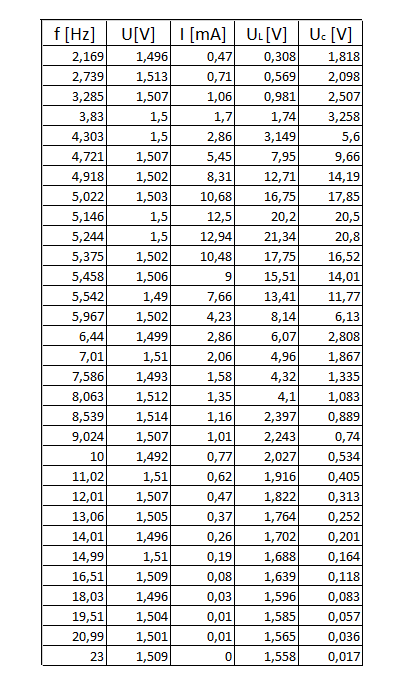
\includegraphics[width=12cm]{tabela.png}
\end{figure}
\newpage

\section{Opracowanie wyników pomiarów}
Zmierzliśmy wstępną maksymalną wartość prądu $I_{max}$ w obwodzie i wynosiła ona $12,94$.
$$$$
Wyznaczyliśmy opór obwodu
$$R = \frac{U_0}{I_{max}}$$

$$R = \frac{1,500}{0,01294} = 115,9196$$
Obliczyliśmy teoretyczną dobroć układu rezonansowego
$$Q_T = \frac{1}{R}\sqrt{\frac{L}{C}}$$ 
$C = 20nF$,  $L=45mh$
$$Q_T = 12,94$$ 
Obliczyliśmy teorytyczną szerokość połówkową krzywej rezonansowej $\Delta f_T$
$$\Delta f_T = \frac{f_T}{Q_T}$$
$$\Delta f_T = \frac{5000}{12,94} = 386,3988$$
Obliczylismy niepewność 
$$u_a = \frac{\delta}{\sqrt{3}} $$
Gdzie $\delta$ to:\\
$1,8\% W + 30\mu A$ niepewność miernika cyfrowego amperomierza,\\
$0,6\% W + 3V$ niepewność miernika cyfrowego woltomierza,\\
$0,1\% W + 3Hz$ niepewność generatora sygnału\\
Sporządziliśmy wykres\\

\begin{figure}
\centering
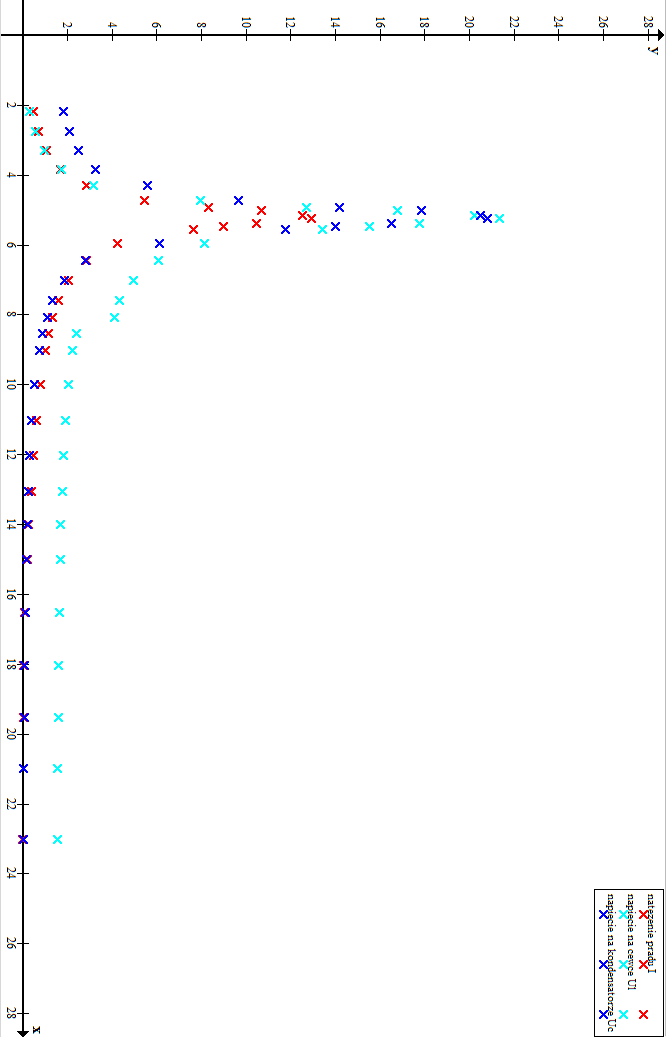
\includegraphics[width=15cm]{wykresrezo.png}
\end{figure}
\newpage

Odczytaliśmy z wykresu częstotliwość rezonansową $f_R$, która wynosi $5,244$\\
Oceniliśmy niepewność $u(f_R)$ która wynosiła $8,244$\\
Metodą szerokości połówkowej krzywej rezonansowej obliczyliśmy dobroć badanego układu rezonansowego 
$$Q=\frac{f_R}{\Delta f} = 13,11$$
$\Delta f = 5440-5040=400Hz$\\
Korzystająć z prawa propagacji niepewności obliczyliśmy niepewność $Q$ oraz $Q_T$\\
$u(U_0)=1,737$\\
$u(I_{max})= 1,866$\\																
$$u(R) = \sqrt{(\frac{u(U_0)}{I_{max}})^2 + (-u(i_{max})\cdot \frac{U_0}{I_{max}^2})^2  } = 0,1352723 $$
$$u(Q_T)= \sqrt{(\sqrt{\frac{L}{C}}\cdot\frac{-u(R)}{R^2})^2} = 0,01510034$$

$$u(Q)=\sqrt{(\frac{-f_r}{(f_2-f_1)^2}u(f_2))^2 + (\frac{f_r}{(f_2-f_1)^2}u(f_1))^2 + (\frac{1}{(f_2-f_1)^2}u(f_r))^2 }= 0,0143578$$\\
Obliczyliśmy teoretyczna  wartość natężenia prądu w rezonansie $I_0$ 
$$I_0= \frac{U_0}{\sqrt{R^2+(\omega L+\frac{1}{\omega C})^2}}=12,94$$
$\omega= 2\pi f_2$
Obliczyliśmy przesunięcie fazowe natężenia prądu względem napięcia wymuszającego

$$cos\phi = \frac{R}{\sqrt{R^2+(2\pi f_r L + \frac{1}{2\pi f_rC})^2}}=1$$

\subsection{Wniosek}
Obliczona teoretyczna wartość natężenia prądu w rezonansie zgadza się z wartością pomiarową. Obliczenia wykazały brak przesunięcia fazowego ponieważ wartość $cos\phi=1$ wynosi $0$
Teoretyczne wartości, które zostały przez nas przyjęte ku naszemu niezadowoleniu były blednę.
Teoretyczna dobroć układu rezonansowego różniła się od wartości obliczonej dobroci.  
Różnice te mogły wynikać z niepewności urządzeń pomiarowych i wahań napięć generatora. 


\end{document}